\section{Probability}

Probability is used to model real-life events and their likelihoods with mathematical tools.

When dealing with probabilities, we want to consider a random process and its possible outcomes. For instance, rolling a dice is a random process that produces six outcomes.

\begin{figure}[H]
    \centering

    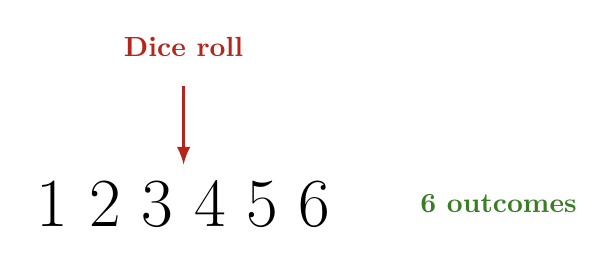
\begin{tikzpicture}
        \node[BrickRed] at (0, 2) {
            \textbf{Dice roll}
        };

        \draw[-latex, very thick, BrickRed] (0, 1.5) -- (0, 0.5);

        \node at (0, 0) {
            \Huge
            \dice{1}
            \dice{2}
            \dice{3}
            \dice{4}
            \dice{5}
            \dice{6}
        };

        \node[OliveGreen] at (4, 0) {
            \textbf{6 outcomes}
        };
    \end{tikzpicture}
    
    \caption{Rolling a dice is a random process that generates six possible outcomes.}
    \label{fig:Ch09-rolling-dice}
\end{figure}

The set of all possible outcomes is called the \textit{sample space} or \textit{universe}, which we denote by \(\Omega\).
%
\[\Omega = \{
    \text{rolling } 1,\;
    \text{rolling } 2,\;
    \text{rolling } 3,\;
    \text{rolling } 4,\;
    \text{rolling } 5,\;
    \text{rolling } 6
\}\]
%
Any subset of \(\Omega\) is called an event. For example, events associated with rolling a dice include the following.
%
\begin{align*}
    A &= \{2, 4, 6\} \tag{rolling an even number}\\
    B &= \{1, 3, 5\} \tag{rolling an odd number}\\
    C &= \{5, 6\} \tag{rolling a number greater than 4}
\end{align*}
%
This allows us to treat events as sets:
%
\begin{align*}
    \text{``Rolling an even number greater than 4''} &= A \cap C \tag{intersection}\\
    \text{``Rolling a number that is odd or greater than 4''} &= B \cup C \tag{union}\\
    \text{``Rolling a number not greater than 4''} &= \overline{C} \tag{complement}\\
    \text{``Rolling an odd number not greater than 4''} &= B \setminus C \tag{minus}
\end{align*}
%
(The complement of a set \(S\) is also sometimes denoted as \(A^c\), but here we will stick to the notation \(\overline{S}\).)

We say that two events \(A\) and \(B\) are \textit{disjoint} if and only if their intersection is the empty set.
%
\[A \cap B = \emptyset\]


\subsection{Probability laws}

We represent the likelihood of an event \(E\) using its probability \(P(E)\). We have the following laws.
%
\begin{align*}
    P(A) &\geq 0 \tag{probabilities are non-negative}\\
    P(\Omega) &= 1 \tag{whole sample space has probability 1}\\
    P(A \cup B) &= P(A) + P(B) \text{\hspace{1em} if \(A, B\) disjoint} \tag{additivity}
\end{align*}
%
This has several consequences, which we will prove below. (Drawing set diagrams are really useful in constructing these proofs.)

\vspace{15pt}
\begin{mdframed}[linewidth=1pt]
\noindent \textbf{Theorem.} If \(A \subseteq B\), then \(P(A) \leq P(B)\).

\textbf{Intuition.} Event \(B\) ``includes'' event \(A\).

\textbf{Proof.} Assume \(A \subseteq B\). Let \(C = B \setminus A\). Since \(A\) and \(C\) are disjoint, we have
%
\begin{align*}
    P(B) &= P(A \cup C) \tag{by definition}\\
    &= P(A) + P(C) \tag{by additivity}\\
    &\geq P(A)\text{.} \tag{\(P(C)\) must be non-negative}
\end{align*}
%
Hence proved.
\end{mdframed}
\vspace{15pt}


\vspace{15pt}
\begin{mdframed}[linewidth=1pt]
\noindent \textbf{Theorem.} \(P(A \cup B) = P(A) + P(B) - P(A \cap B)\).

\textbf{Proof.} Let \(A' = A \setminus B\) and \(B' = B \setminus A\). It follows that
%
\begin{align*}
    \text{RHS} &= P(A) + P(B) - P(A \cap B)\\
    &= P(A) + P(B' \cup (A \cap B)) - P(A \cap B)\\
    &= P(A) + P(B') + P(A \cap B) - P(A \cap B) \tag{\(B'\) and \(A \cap B\) are disjoint}\\
    &= P(A) + P(B')\\
    &= P(A \cup B') \tag{\(A\) and \(B'\) are disjoint}\\
    &= P(A \cup B)\\
    &= \text{LHS}
\end{align*}
%
Hence proved.
\end{mdframed}
\vspace{15pt}



\vspace{15pt}
\begin{mdframed}[linewidth=1pt]
\noindent \textbf{Theorem.} \(P(\overline{A}) = 1 - P(A)\).

\textbf{Proof.} Since \(A\) and \(\overline{A}\) are disjoint, we have
%
\begin{align*}
    P(A \cup \overline{A}) &= P(A) + P(\overline{A})\\
    P(\Omega) &= P(A) + P(\overline{A})\\
    1 &= P(A) + P(\overline{A})\\
    P(\overline{A}) &= 1 - P(A)
\end{align*}
%
Hence proved.
\end{mdframed}
\vspace{15pt}



\subsection{Discrete and continuous probabilities}

A set is said to be \textit{countable} if it is finite or in bijection with \(\mathbb{N}\).


\subsubsection{Discrete probabilities in countable sample spaces}

By the law of additivity for disjoint events, if the sample space of a random process is countable, we can measure probabilities in that space as a sum.
%
\[P(A) = \sum_{a \in A}\; P(\{a\})\]

For example, in our example of dice rolling, let \(C\) be the event of rolling a number greater than \(4\). This event consists of two possible outcomes: rolling a \(5\) and rolling a \(6\). Therefore,
%
\begin{align*}
    P(C) &= P(\{
        \text{rolling } 5,\;
        \text{rolling } 6
    \})\\
    &= P(\{\text{rolling } 5\})
    + P(\{\text{rolling } 6\})\\
    &= \frac{1}{6} + \frac{1}{6}\\
    &= \frac{1}{3}
\end{align*}

Furthermore, in the case where \(\Omega\) has a finite size \(n\) with every outcome equally likely (e.g. dice rolling), we can express the probability of any event \(A\) as
%
\[P(A) = \frac{\abs{A}}{n}\text{.}\]
%
This streamlines the calculation of \(P(C)\) above as follows.
%
\[
    P(C) = P(\{
        \text{rolling } 5,\;
        \text{rolling } 6
    \})
    = \frac{2}{6} = \frac{1}{3}
\]

Now consider a different scenario with an infinite, but nevertheless still countable sample space.

\begin{quote}
    A fair coin is tossed repetitively until heads is observed. The number of coin tosses is recorded as the outcome of this experiment. The sample space \(\Omega\) of this process is thus \(\mathbb{N}\), which is countably infinite.
    
    Verify that \(P(\Omega) = 1\).
\end{quote}

Since the sample space is countably infinite, we can express \(P(\Omega)\) as an infinite sum.
%
\begin{align*}
    P(\Omega) &= \Sigma_{a \in \Omega}\; P(\{a\})\\
    &= P(\{1\}) + P(\{2\}) + P(\{3\}) + \cdots\\
    &= P(\text{First head on toss \#1}) + P(\text{First head on toss \#2}) + P(\text{First head on toss \#3}) + \cdots\\
    &= \frac{1}{2} + \frac{1}{2} \times \frac{1}{2} + \frac{1}{2} \times \frac{1}{2} \times \frac{1}{2} + \cdots\\
    &= \sum_{k\geq 1} \frac{1}{2^k}\\
    &= 1 \tag{geometric series}
\end{align*}



\subsubsection{Continuous probabilities in uncountable sample spaces}

If the sample space is instead \textit{uncountable} (e.g. intervals of \(\mathbb{R}\)), then we can only measure probabilities as a continuous sum, i.e. an integral.

For example, consider a random number \(x\) in the interval \([0, 1]\). The probabiliy that \(x\) is strictly higher than \(0.7\) is given by
%
\[P(x > 0.7) = \int_{0.7}^{1} dx = 0.3\text{.}\]



\subsection{Conditional probabilities}

Conditional probabilities help us reason about the probability of an event under the assumption that another event took place.

The probability of \(A\) given \(B\), denoted as \(P(A \vert B)\), is given by
%
\[P(A\vert B) = \frac{P(A \cap B)}{P(B)}\text{.}\]

This gives us two important properties: the law of total probability and Bayes' theorem.

(Since both of these properties can be easily proved using the definition of conditional probability given above, below we will focus more on gaining an intuitive understanding of these laws rather than simply showing that they are mathematically true.)


\subsubsection{Law of total probability}

The law of total probability states that
%
\[P(B) = {\color{BrickRed} P(A) \cdot P(B \vert A)} + {\color{MidnightBlue} P(\overline{A}) \cdot P(B \vert \overline{A})}\]
%
which is equivalent to
%
\[P(B) = {\color{BrickRed} \underbrace{P(A \cap B)}_{A \text{ \& } B \text{ both happen}}} + {\color{MidnightBlue} \underbrace{P(\overline{A} \cap B)}_{B \text{ happens but } A \text{ doesn't}}} \text{.}\]

As an example, consider the following scenario.
%
\begin{quote}
    \textbf{Scenario.}

    Depending on how well they work, ovens can either be classified as into two categories.
    
    \begin{figure}[H]
        \centering
        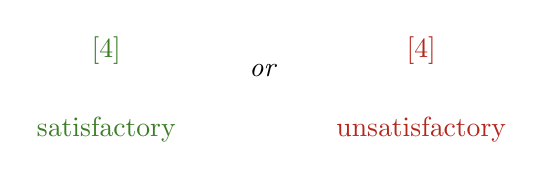
\begin{tikzpicture}
            \node[OliveGreen] at (-2, 0) {\oven[4]};
            \node[OliveGreen] at (-2, -1) {satisfactory};
    
            \node at (0, -0.25) {\textit{or}};
    
            \node[BrickRed] at (2, 0) {\oven[4]};
            \node[BrickRed] at (2, -1) {unsatisfactory};
        \end{tikzpicture}
    \end{figure}
    
    Suppose that \(60\%\) of ovens available on the market are supplied by company A, while the other \(40\%\) are supplied by company B. The percentage of satisfactory ovens produced is \(90\%\) for company A and \(80\%\) for company B.

    \begin{figure}[H]
        \centering
        
\begin{tikzpicture}
            \node[BurntOrange, draw, very thick, fill=BurntOrange!10, inner sep=3mm] at (-1, 0) {\Huge \(\mathcal{A}\)};
    
            \node[MidnightBlue, draw, very thick, fill=MidnightBlue!10, inner sep=3mm] at (1, 0) {\Huge \(\mathcal{B}\)};
        \end{tikzpicture}
    \end{figure}

    You have just purchased an oven. What is the probability that it is satisfactory?
\end{quote}

To answer this question, we consider a representative sample of ovens available on the market, where \(60\%\) of ovens are from company A and the other \(40\%\) are from company B. This is shown in figure \ref{fig:Ch09-ovens-1}.

Take into account the satisfactory percentage for each company results in figure \ref{fig:Ch09-ovens-2}.

\begin{figure}[H]
    \centering
    \begin{tikzpicture}[scale=0.95]
        \foreach \x in {0,...,5} {
            \foreach \y in {0,...,9} {
                \node[BurntOrange, draw, fill=BurntOrange!7.5] at (\x, \y) {\color{black}\oven[2]};
            }
        }

        \foreach \x in {6,...,9} {
            \foreach \y in {0,...,9} {
                \node[MidnightBlue, draw, fill=MidnightBlue!7.5] at (\x, \y) {\color{black}\oven[2]};
            }
        }

        \draw [decorate, decoration={calligraphic brace, mirror, amplitude=5pt}, pen colour={BurntOrange}, ultra thick] (-0.5, -0.5) --  (5.5, -0.5) node[pos=0.5,below=5pt,BurntOrange]{Company A (\(60\%\))};

        \draw [decorate, decoration={calligraphic brace, mirror, amplitude=5pt}, pen colour={MidnightBlue}, ultra thick] (5.5, -0.5) --  (9.5, -0.5) node[pos=0.5,below=5pt, MidnightBlue]{Company B (\(40\%\))};
    \end{tikzpicture}
    \caption{A representative sample (of size 100) of ovens available on the market. \(60\%\) of ovens are from company A and the other \(40\%\) are from company B.}
    \label{fig:Ch09-ovens-1}
\end{figure}

\begin{figure}[H]
    \centering
    \begin{tikzpicture}[scale=0.95]
        \foreach \x in {0,...,5} {
            \foreach \y in {0,...,8} {
                \node[BurntOrange, draw, fill=BurntOrange!7.5] at (\x, \y) {\color{OliveGreen}\oven[2]};
            }
        }

        \foreach \x in {0,...,5} {
            \foreach \y in {9} {
                \node[BurntOrange, draw, fill=BurntOrange!7.5] at (\x, \y) {\color{BrickRed}\oven[2]};
            }
        }

        \foreach \x in {6,...,9} {
            \foreach \y in {0,...,7} {
                \node[MidnightBlue, draw, fill=MidnightBlue!7.5] at (\x, \y) {\color{OliveGreen}\oven[2]};
            }
        }

        \foreach \x in {6,...,9} {
            \foreach \y in {8,9} {
                \node[MidnightBlue, draw, fill=MidnightBlue!7.5] at (\x, \y) {\color{BrickRed}\oven[2]};
            }
        }

        \draw [decorate, decoration={calligraphic brace, mirror, amplitude=5pt}, pen colour={BurntOrange}, ultra thick] (-0.5, -0.5) --  (5.5, -0.5) node[pos=0.5,below=5pt,BurntOrange]{Company A (\(60\%\))};

        \draw [decorate, decoration={calligraphic brace, mirror, amplitude=5pt}, pen colour={MidnightBlue}, ultra thick] (5.5, -0.5) --  (9.5, -0.5) node[pos=0.5,below=5pt, MidnightBlue]{Company B (\(40\%\))};

        \draw [decorate, decoration={calligraphic brace, amplitude=5pt}, ultra thick] (-0.6, -0.5) --  (-0.6, 8.5) node[pos=0.5,left=5pt, text width=2.5cm, align=center]{Company A's satisfactory percentage \(=90\%\)};

        \draw [decorate, decoration={calligraphic brace, amplitude=5pt, mirror}, ultra thick] (9.6, -0.5) --  (9.6, 7.5) node[pos=0.5,right=5pt, text width=2.5cm, align=center]{Company B's satisfactory percentage \(=80\%\)};
    \end{tikzpicture}
    \caption{An illustration of the law of total probability.}
    \label{fig:Ch09-ovens-2}
\end{figure}

From figure \ref{fig:Ch09-ovens-2}, it is apparent that
%
\begin{align*}
    &\; P(\text{satisfactory})\\
    =&\; P(\text{from A}) \cdot P(\text{A's satisfactory percentage}) + P(\text{from B}) \cdot P(\text{B's satisfactory percentage})\\
    =&\; P(\text{from A}) \cdot P(\text{satisfactory} \;\vert\; \text{from A}) + P(\text{from B}) \cdot P(\text{satisfactory} \;\vert\; \text{from B})\\
    =&\; P(\text{from A}) \cdot P(\text{satisfactory} \;\vert\; \text{from A}) + P(\overline{\text{from A}}) \cdot P(\text{satisfactory} \;\vert\; \overline{\text{from A}})
\end{align*}
%
which is equivalent to applying the law of total probability!





\subsubsection{Bayes' theorem}

Bayes' theorem states the following.
%
\begin{align*}
    P(A \vert B) &= \frac{P(B \vert A) P(A)}{P(B)}\\
    &= \frac{P(B \vert A) P(A)}{P(B)}\\
\end{align*}
%
Again we want to consider a concrete, tangible scenario.


\begin{quote}
    \textbf{Scenario.}

    Assume that \(2\%\) of women worldwide are pregnant at any given time.

    A recently developed pregnancy test kit is shown to give the following results.
    %
    \begin{itemize}
        \item \textbf{True positives:} For pregnant women, the kit correctly detects a pregnancy \(99 \%\) of the time.
        \item \textbf{False positives:} For those who are not pregnant, the kit incorrectly shows a positive result \(5\%\) of the time.
    \end{itemize}
    %
    A woman using this pregnancy test has just received a positive result. What is the probability that she is indeed pregnant?
\end{quote}

Notice that we are given information about
%
\[P(\text{positive} \;\vert\; \text{pregnant})\]
%
and are asked to evaluate
%
\[P(\text{pregnant} \;\vert\; \text{positive}) \text{.}\]
%
This flip between given and desired information indicates that Bayes' theorem might be helpful.

Using Bayes' theorem, we have
%
\begin{align*}
    &\; P(\text{pregnant} \;\vert\; \text{positive})\\
    =&\; \frac{P(\text{positive} \;\vert\; \text{pregnant}) \cdot P(\text{pregnant})}{P(\text{positive})}\\
    =&\; \frac{P(\text{positive} \;\vert\; \text{pregnant}) \cdot P(\text{pregnant})}{P(\text{pregnant}) \cdot P(\text{positive} \;\vert\; \text{pregnant}) + P(\text{not pregnant}) \cdot P(\text{positive} \;\vert\; \text{not pregnant})} \tag{law of total probability}\\
    =&\; \frac{0.99 \cdot 0.02}{0.99 \cdot 0.02 + (1 - 0.02) \cdot 0.05}\\
    =&\; \frac{99}{244} \approx 28.8\%
\end{align*}
%
which seems counterintuitively low, but is actually correct! See figure \ref{fig:Ch09-pregnancies} for a visualisation.

\begin{figure}[H]
    \centering
    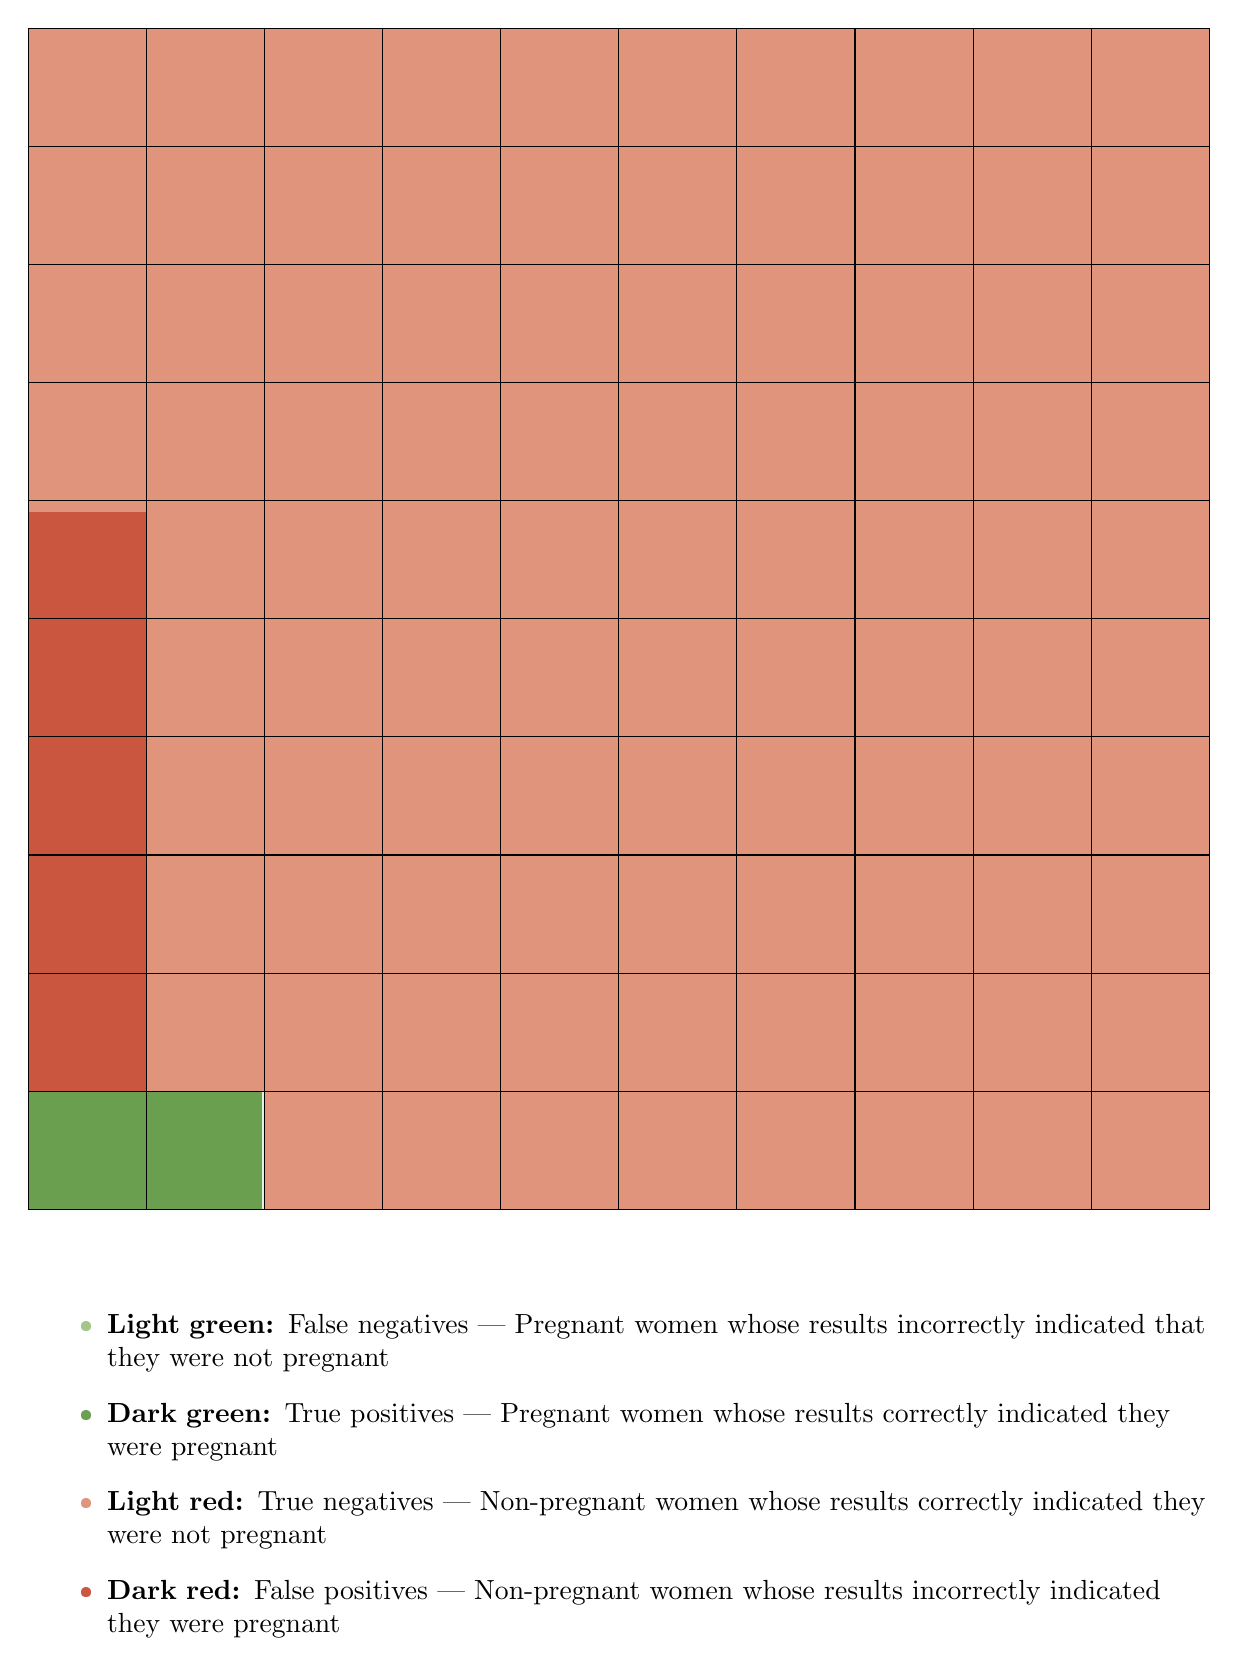
\begin{tikzpicture}[scale=1.5]
        \foreach \x in {0,...,9} {
            \foreach \y in {0,...,9} {
                \fill[BrickRed!40] (\x, \y) rectangle (\x+1, \y+1);
            }
        }

        \foreach \x in {0,1} {
            \foreach \y in {0} {
                \fill[OliveGreen!10] (\x, \y) rectangle (\x+1, \y+1);
            }
        }

        \fill[OliveGreen!70] (0, 0) rectangle (2*0.99, 1);
        \fill[BrickRed!70] (0, 1) rectangle (1, 5.9);

        \foreach \x in {0,...,9} {
            \foreach \y in {0,...,9} {
                \draw (\x, \y) rectangle (\x+1, \y+1);
            }
        }

        \node[text width=15cm, align=left, anchor=north west] at (0, -0.5) {
            \begin{itemize}
                \item[\textcolor{OliveGreen!40}{\textbullet}]  \textbf{Light green:} False negatives --- Pregnant women whose results incorrectly indicated that they were not pregnant
                \item[\textcolor{OliveGreen!70}{\textbullet}] \textbf{Dark green:} True positives --- Pregnant women whose results correctly indicated they were pregnant
                \item[\textcolor{BrickRed!40}{\textbullet}] \textbf{Light red:} True negatives --- Non-pregnant women whose results correctly indicated they were not pregnant
                \item[\textcolor{BrickRed!70}{\textbullet}] \textbf{Dark red:} False positives --- Non-pregnant women whose results incorrectly indicated they were pregnant
            \end{itemize}
        };
    \end{tikzpicture}
    \caption{Bayes' theorem, illustrated using pregnancy test kits as an example. Each of the 100 squares above depicts a woman. For pregnant women, the kit correctly detects a pregnancy \(99 \%\) of the time; for those who are not pregnant, the kit incorrectly shows a positive result \(5\%\) of the time.}
    \label{fig:Ch09-pregnancies}
\end{figure}


\subsubsection{Independent events}

Two events \(A\) and \(B\) are said to be \textit{independent} if we have
%
\[P(A \cap B) = P(A) \cdot P(B)\text{.}\]
%
This is equivalent to either of the following equations.
%
\begin{align*}
    P(A \vert B) &= P(A)\\
    P(B \vert A) &= P(B)
\end{align*}



\subsection{What are random variables?}

So far we've been talking about probabilities with respect to events and random processes, but how can these ideas be properly formalised?

We represent a random process as a \textit{random variable} \(X\) that maps each possible outcome to its corresponding probability\footnote{Although the word ``variable'' is used, a random variable is actually a function.}.
%
\[X: \Omega \mapsto [0, 1]\]
%
We use the notation \(P(X = a)\) to denote the probability of the outcome of the random process being \(a\).

Here, we will introduce two types of random variables.


\subsubsection{Bernoulli random variables}

A \textit{Bernoulli random variable} is one that can only produce the values \(0\) or \(1\). The probabilities of \(0\) and \(1\) being generated do not have to be equal. This means that defining a Bernoulli random variable requires a parameter \(p\), where \(0 \leq p \leq 1\).
%
\begin{align*}
    P(X = 1) &= p\\
    P(X = 0) &= 1-p
\end{align*}
%
Examples include:
%
\begin{itemize}
    \item The result of tossing a fair coin.
    \item The result of tossing an unfair coin.
    \item Rolling a 20-sided dice and checking if the resultant number is prime.
\end{itemize}



\subsubsection{Binomial random variables}

Consider a Bernoulli random variable (with parameter \(p\)). Suppose we repeatedly check its outcome \(n\) times, and count the number of \(1\)s produced. In other words, we compute the sum of \(n\) independent Bernoulli variables with parameter \(p\)

This sum is called a \textit{binomial random variable}, which takes the parameters \(n\) and \(p\). Combinatorics\footnote{Note that the ``choose'' function \(C^n_k\) can also be denoted as \(\begin{bmatrix} n\\k \end{bmatrix}\).} tell us that
%
\[P(X = k) = C^n_k p^k (1-p)^{n-k}\text{.}\]
%


\subsection{Expected value}

Given a random variable \(X\), we define its \textit{expected value}\footnote{Also called the \textit{mean}.} \(E(X)\) as the average of all its possible resultant values, weighted using the corresponding probabilities.
%
\[E(X) = \Sigma_{x \in \Omega} x \cdot P(X = x)\]

Expected values have the property that for any two random variables \(X\) and \(Y\), we have
%
\[E(X + Y) = E(X) + E(Y)\text{.} \tag{additivity}\]

For example, let \(X\) be a Bernoulli variable with parameter \(p\). Its expected value is
%
\begin{align*}
    E(X) &= 1 \cdot p + 0 \cdot (1 - p)\\
    &= p\text{.}
\end{align*}

Now consider a binomial random variable \(Y\) with parameters \(n\) and \(p\). Its expected value is given by
%
\begin{align*}
    E(Y) &= E(\underbrace{\text{Bernoulli}(p) + \text{Bernoulli}(p) + \cdots + \text{Bernoulli}(p)}_{n \text{ times}})\\
    &= \underbrace{E(\text{Bernoulli}(p)) + E(\text{Bernoulli}(p)) + \cdots + E(\text{Bernoulli}(p))}_{n \text{ times}}\\
    &= \underbrace{p + p + \cdots + p}_{n \text{ times}}\\
    &= np\text{.}
\end{align*}



\subsection{Variance and standard deviation}

We define the \textit{variance} of a random variable \(X\) as
%
\[\text{Var}(X) = E((X - E(X))^2)\]
or
%
\[\text{Var}(X) = E(X^2) - (E(X))^2\text{.}\]
%
This represents the expected squared distance of an outcome from \(X\)'s expected value.

For example, a Bernoulli variable \(X\) with parameter \(p\) has variance
%
\begin{align*}
    \text{Var}(X) &= E(X^2) - (E(X))^2\\
    &= E(X) - (E(X))^2 \tag{\(0^2 = 0\) and \(1^2 = 1\)}\\
    &= p - p^2\\
    &= p(1 - p)
\end{align*}

The \textit{standard deviation} \(\sigma\) of a random variable is defined as the square root of its variance.



\subsection{Normal distribution}

So far we have only seen discrete random variables, where the universe is a countable set.

For continuous random variables (e.g. when the outcome is within an interval on the number line), we must calculate probabilities using integrals.
%
\[P(X \in [a, b]) = \int_a^b f(x) \,dx\]

A \textit{normal distribution} a type of distribution for real-valued, continuous random variables. It is based on the function \(x = e^{-x^2}\).

The normal distribution takes two parameters:
%
\begin{itemize}
    \item The mean \(\mu\) (i.e. the expected value)
    \item The standard deviation \(\sigma\)
\end{itemize}
%
and is parameterised as follows:
%
\[P(X \in [a, b]) = \int_a^b \frac{1}{\sigma \sqrt{2\pi}} e^{-\frac{1}{2} (\frac{x - \mu}{\sigma})^2} \;dx\]
%
where the constant \(1/{\sigma \sqrt{2\pi}}\) is used to normalise the integral, ensuring that the area under the graph equals \(1\), since \(P(\Omega) = 1\). Note that integrals of this form do not have closed form solutions. This means they can only be estimated using numerical methods.

See figure \ref{fig:Ch09-normal-distribution}.

\begin{figure}[H]
    \centering
    \includegraphics[width=0.7\textwidth]{Images/NormalDistribution.png}
    \caption{Examples of normal distributions. The parameters \(\mu\) and \(\sigma^2\) represent the mean and variance respectively.}
    \label{fig:Ch09-normal-distribution}
\end{figure}

Consider for example the following scenario.

\begin{quote}
    \textbf{Scenario.}

    Intelligence is often assumed to be normally distributed among a population. Therefore, a person's intelligence quotient (IQ) is defined in such a way that it fits a normal distribution with mean \(\mu = 100\) and standard deviation \(\sigma = 15\).

    What is the probability that a randomly selected individual has an IQ between \(120\) and \(140\)?
\end{quote}

We can answer this by evaluating the following integral.
%
\begin{align*}
    \int_{120}^{140} \frac{1}{\sigma \sqrt{2\pi}} e^{-\frac{1}{2} (\frac{x - \mu}{\sigma})^2} \;dx
    &= \int_{120}^{140} \frac{1}{15 \sqrt{2\pi}} e^{-\frac{1}{2} (\frac{x - 100}{15})^2} \;dx\\
    &\approx 0.08738 \tag{by numerical methods}
\end{align*}
